\documentclass[twocolappendix, appendixfloats, numberedappendix, twocolumn, apj]{openjournal}

\usepackage{graphicx}
\usepackage{latexsym,amssymb}
\usepackage{amsmath,morefloats}
\usepackage[backref,breaklinks,colorlinks,citecolor=blue]{hyperref}
\usepackage{natbib,graphicx,amsmath,subfigure,color,xcolor}
\usepackage{verbatim}
\usepackage{threeparttable}
\usepackage{xspace}

\newcommand{\ess}[1]{\textcolor{red}{[ESS: \bf #1]}\xspace}
\newcommand{\mrb}[1]{\textcolor{purple}{[MRB: \bf #1]}\xspace}

\newcommand{\mdet}{\textsc{metadetection}\xspace}
\newcommand{\mcal}{\textsc{metacalibration}\xspace}
\newcommand{\galsim}{\textsc{galsim}\xspace}
\newcommand{\descwl}{\textsc{WeakLensingDeblending}\xspace}
\newcommand{\ngmix}{\textsc{ngmix}\xspace}
\newcommand{\sep}{\textsc{sep}\xspace}
\newcommand{\ksigma}{\mbox{\boldmath $\mathrm{K}_{\sigma}$}\xspace}
\newcommand{\pgauss}{\texttt{pgauss}\xspace}

\shorttitle{Pre-PSF Moments for Weak Lensing Shear Measurement}
\shortauthors{Becker \& Sheldon}

\begin{document}
\title{Pre-PSF Moments for Weak Lensing Shear Measurement}

\author{Matthew R. Becker}
\affil{High Energy Physics Division, Argonne National Laboratory, Lemont, IL 60439, USA}
\author{Erin S. Sheldon}
\affil{Brookhaven National Laboratory, Bldg 510, Upton, New York 11973, USA}
% \author{Eli Rykoff}
% \affil{}

\begin{abstract}
  We present a technique to measure pre-PSF, aperture-matched weighted fluxes, sizes,
  and shapes of extended astronomical objects. Our technique directly deconvolves the
  PSF from the image of the object and then estimates real-space moments of the object
  using direct integrals in Fourier-space against the appropriate transformations of the
  moment weight functions. This measurement pipeline for a Gaussian weight function,
  which we call \pgauss, executes quickly, O(10 ms) \mrb{check this again}, and
  deterministically, requiring only two fast-fourier transforms (FFTs) and some sums
  over the results. This pipeline additionally includes zero-padding and apodization
  corrections in order to control FFT artifacts which can arise during the
  deconvolution. We demonstrate that for isolated objects, we can recover the underlying
  true aperture flux to better than a fraction of a percent and report flux errors that
  are accurate to better than a few percent. We additionally estimate the optimal
  aperture for Vera C. Rubin Observatory weak lensing studies ($\approx1.5$'' FWHM) and
  demonstrate that the \mdet weak lensing shear estimator is unbiased when coupled with
  the \pgauss shape estimate. Due to the fact that our measurement aperture is fixed,
  the colors of objects measured with \pgauss fluxes are suitable for photometric
  redshift estimation as well. Our implementation is available in the \texttt{ngmix}
  software package.
\end{abstract}

\section{Introduction}\label{sec:intro}

The measurement of extended objects in astronomical images is a complicated subject with a long
history. The fundamental ambiguity in these measurements is how to declare an "end" to the object
and the start of the background. There are two general approaches to resolving this ambiguity. The
first approach is to set the measurement aperture via some criterion (e.g., a fixed aperture size,
a particular isophote, etc.) \mrb{cite}. The second approach is to rely on a model of the underlying object to
essentially extrapolate the amount of flux at or below the background level \mrb{cite}. Each of these approaches
have advantages and disadvantages related to not only their performance for specific analysis tasks
like photometric calibration or photometric redshift measurement, but also related to their speed and
reliability.

Another fundamental ambiguity in these measurements is the blending of objects along the line-of-sight. This topic
is of particular interest to next-generation surveys like the Vera C. Rubin Observatory
Legacy Survey of Space and Time (LSST) due to the high fraction of objects that will be blended in Rubin
data due to its depth \mrb{cite}. A variety of approaches to handling blending have been devised using
model fits, the symmetries of the underlying objects, or both \mrb{}. Notably techniques powered by deep
neural network architectures \mrb{cite} appear to show considerable promise due to their ability to learn
complex priors about the diversity of astronomical objects.

In addition to the physical ambiguities above, there are a number of important but more practical considerations in these measurements. First,
modern astronomical surveys take many images of the same object in one or more pass bands. Any object
measure needs to be able to account for the varying background levels and point-spread functions (PSFs)
of the resulting dataset. Second, most modern cosmological surveys seek to use photometric redshifts as a
key part of their analyses \mrb{cite}. For this specific analysis task, the effective aperture used in the
measurement needs to be matched across different pass bands in order to obtain reliable object colors. Third,
in modern cosmological surveys the objects are interest are generally low signal-to-noise and small. In this
regime, complex model fitting methods need non-trivial priors or other tricks \mrb{cite SDSS, DES} in order
to achieve stability. Finally, measurement speed, reliability/stability, and the ability to parallelize the
code are important considerations for the datasets of billions of objects expected from surveys like the LSST.
Even small measurement failure rates or small increases in running time can lead to large absolute changes
in the cost and quality of the final data processing results.

In this work, we describe the performance of a technique that uses a fixed weight function applied to
the pre-PSF object in real-space to define the measurement aperture. With this weight function, we compute a set of
real-space moments of the object's surface brightness profile, giving the flux, centroid, size, and shape. This technique is
motivated by modern weak lensing shear measurement pipelines which require that the selection of objects
in terms of their colors, sizes, and overall fluxes be done within the weak lensing measurement pipeline
\mrb{cite} in order to control for shear selection effects. With this motivation in mind, our technique
directly deconvolves the PSF from the object's image and then works entirely in Fourier-space to estimate
the real-space moments. The measurement aperture can be fixed across bands, generating high-quality object
colors for photometric redshift inference. The pipeline is also easily parallelized since the moments can be combined
at the catalog level after extraction from the images. The technique, which we call \pgauss when used with a
Gaussian aperture, is inspired by the Fourier-space moments of the Bayesian Fourier Domain shear measurement
method of \mrb{cite}. This technique is also closely related to the \texttt{GaaP} method of \mrb{cite} which
takes a somewhat similar approach using Shapelet expansions \mrb{cite}.

Notably, obtaining reliable results with this technique requires careful attention to numerical
artifacts, especially when performing the PSF deconvolution. We implement a variety of corrections including
zero-padding and apodization to ensure stability. We also require that the final real-space measurement
aperture be somewhat larger than the image PSF in order to suppress noise from the PSF deconvolution. This
requirement is a fundamental trade-off since it can reduce the signal-to-noise of the overall measurement.
In practice, this effect is small since the majority of objects suitable for a weak lensing
analysis are small in the first place.

Finally, in this work we largely ignore the effects of object blending for several reasons. First,
object blending effects are largely common across the class of fixed aperture measurement methods.
For example, a small object on top of a much larger background object will always have its flux boosted
by a similar overall factor regardless of the specific choice of fixed measurement aperture. Second,
most techniques to handle blending involve complicated model fitting, which is well beyond the scope
of this work. Lastly, the weak lensing shear measurement technique that primarily motivates this work,
\mdet, is insentiive to object blending.

Our paper is arranged as follows. In ...

\section{Pre-PSF Moment Measurement in Fourier-space}

In this section, we introduce our core methodology for computing fast, pre-PSF real-space moment
measures. It depends on the follow properties of Fourier transforms:
\begin{enumerate}
\item The Fourier transform of a quantity like $x^2W(x)$ is $\propto\frac{d^{2}W(k)}{dk^2}$.
\item The integral of the product of two functions in real-space can be computed from their Fourier
      transforms: $\int dx^2 I(x)W(x) = \int dk^2 I(k)W(k)$. This relation is called the Plancherel theorem.
\end{enumerate}
Putting the relationships together, we can compute the non-central moments of the profile of
an image via
\begin{eqnarray}
f                          & = \int dx^2 I(x)W(x) =            & \int dk^2 I(k)W(k) \\
\langle x_{i} \rangle      & = \int dx^2 x_{i} I(x)W(x) =      & \int dk^2 I(k)\frac{dW(k)}{dk_i} \\
\langle x_{i}x_{j} \rangle & = \int dx^2 x_{i}x_{j} I(x)W(x) = & \int dk^2 I(k)\frac{dW(k)}{dk_{i}dk_{j}}\,.
\end{eqnarray}
With the above we can measure pre-PSF, real-space moments as follows:
\begin{enumerate}
\item Given an image of a galaxy $I(x)$ and the PSF $P(x)$, deconvolve the PSF in Fourier-space.
\item Pick a filter function $W(x)$ that is large enough to suppress any noise from modes increased
      during the PSF deconvolution.
\item Use the relationships above to measure the moments and shape of the object through sums in Fourier-space.
\end{enumerate}
Following \mrb{cite}, we define the follow quantities from the moments above
\begin{eqnarray}
M_{f} & = & f \nonumber \\
M_{x_1} & = & \langle x_{1} \rangle/f \nonumber \\
M_{x_2} & = & \langle x_{2} \rangle/f \nonumber \\
T & = & (\langle x_{1}x_{1} \rangle + \langle x_{2}x_{2} \rangle)/f \nonumber \\
M_{+} & = & (\langle x_{1}x_{1} \rangle - \langle x_{2}x_{2} \rangle)/f \nonumber \\
M_{\times} & = & 2 \langle x_{1}x_{2} \rangle/f\ . \nonumber
\end{eqnarray}
We can define shape measures through $e_1 = M_{+}/T$ and $e_2 = M_{\times}/T$. The errors in the
moments are computed through error propagation through the linear operations above assuming
the pixel noise is uncorrelated in real-space between adjacent pixels. The errors on the shapes
$e_{1,2}$ are also computed via error propagation, but note that their error distributions can have
large tails due to the division by $T$.

There are a fair number of technical details in the implementation that help to make it efficient and
accurate. These are discussed below.

\subsection{Weight Function Choices}

We've implemented two weight function choices. The first is a symmetric Gaussian weight
function with a given full-width-at-half-maximum. We call our estimator with a Gaussian
kernel \pgauss. The second choice is a compact filter
in Fourier-space that we call \ksigma and was introduced by \citet{BernBFD2016}:
\begin{equation}
\label{ksigma}
W\left(|k^2|\right)  \equiv \left\{
\begin{array}{cc}
\left( 1 - \frac{k^2\sigma^2}{2N}\right)^N & k <
                                             \frac{\sqrt{2N}}{\sigma} \\
0 & k \ge
                                             \frac{\sqrt{2N}}{\sigma}
\end{array}
\right.
\end{equation}
Following \citet{BernBFD2016}, we take $N = 4$, which makes the weight a good
approximation to a gaussian.  This weight has the nice property that it goes
smoothly to zero at a chosen value of $k$. Optimizing the the measurement aperture
is non-trivial and discussed below.

\subsection{Implementation Details}

We've had to handle several technical details on the implementation in order to get
reliable and fast results. We describe and address these things one-by-one here.

\textbf{Zero-padded FFTs} The FFTs used for implementing the steps above assume that
the image is periodic. As this is never the case in real data, we zero-pad the FFTs by a
factor of four.

\textbf{Apodization} Real astronomical images can have non-zero mean background levels
due to blending of a small object on top of a larger one, errors in sky subtraction,
the bright wings of stars, etc. After zero-padding, the non-zero background level appears
as a sharp change in the image when moving over the edge of the stamp. This sharp feature
can cause artifacts in the FFTs, especially when deconvolving by the PSF. To prevent this,
we smoothly scale the image down to zero over the edge of the stamp using a cumulative triweight
apodization kernel:
\begin{equation}
T(y) = \left\{
\begin{array}{cc}
0 & y < -3 \\
(-5y^7 / 69984 & \\
+ 7y^5 / 2592 & \\
- 35y^3 / 864 & -3 \le y \le 3 \\
+ 35y / 96 & \\
+ 1 / 2) &  \\
1 & y > 3
\end{array}
\right.
\end{equation}
with $y = (x-m)/h + 3$. Here $x$ is the pixel location in the image, $m=6h$ is the maximum
apodization region, and $h$ is the kernel width parameter. This kernel is applied so that it starts
at zero at the edge of the image and goes to unity at $6h$ pixels inside the image. The exact shape
of this kernel doesn't matter as long as it is sufficiently slowly varying compared to the PSF.
We use $h=1.5$ pixels which is sufficient for a typical ground-based survey.

\textbf{PSF Deconvolution} We deconvolve the PSF in Fourier-space. In order to avoid dividing by
zero, we truncate the PSF to $10^{-5}$ of its maximum Fourier amplitude. The estimators in this work
become unstable if the moments aperture is too small in real-space and these Fourier modes are not truncated.

\textbf{WCS Handling} We require that the PSF and the image have the same WCS Jacobian
and that this Jacobian is constant across the image. We remove the WCS by mapping pixel locations
in Fourier-space to the Fourier-space WCS tangent plane before computing the moments kernels.
We correct for overall shifts in the centers of the image and the PSF though phase factors applied
in Fourier-space, but in image pixel coordinates.

\textbf{Error Propagation} We compute the errors in our measurements by directly computing the
covariance in Fourier-space. Due to the fact that all of the operations for computing the moments
above are linear, we can do this operation analytically. As shown below, our reported errors are
accurate to better than a few percent for isolated objects.

\textbf{Efficiency} Our final implementation requires two FFTs, uses \texttt{numba} to compute the
apodization masks, uses use a fast exponential implementation that is accurate to float precision,
and takes advantage of Fourier-space modes that are set to zero by the moments weight function by ignoring
them early on in the code. Overall, it runs at a speed of ${\cal O}(10s)$ of milliseconds per
object depending on the stamp size \mrb{check this again}. Our implementation is available in the
\texttt{ngmix} software package.

\subsection{Adaptive Pre-PSF Moments}

We can extend our technique to compute adaptive pre-PSF moments as well. Our algorithm is exactly like
the original adaptive moments algorithm \mrb{cite}, except that we modify the weight function at each step
in order to force it to smoothly approach a round, minimum sized Gaussian weight as the size of the
kernel gets smaller. This modification is needed to control the noise in our moments estimates due to
PSF deconvolution. Specifically, the weight function shape $e_{1,2}$ and $T$ is transformed as

\begin{eqnarray}
f & = & {\cal S}(T/(1 + 2 |e|), T_{\rm min}, \Delta_T) \\
e_{1,2} & \rightarrow & f \times e_{1,2} \\
T & \rightarrow & fT + (1-f)T_{\rm min}
\end{eqnarray}
where $T_{\rm min}$ is the minimum allowed kernel size and $\Delta_T$ specifies the region over which
the function ${\cal S}(T, T_{\rm min}, \Delta_T)$ goes from 0 when $T=T_{\rm min}$ to 1 at $T\geq T_{\rm min} + \Delta_T$.
We use the same cumulative triweight kernel as above with $h=\Delta_T/6$ and the mean adjust to satisfy the limiting
behavior for ${\cal S}$.

\section{Results}

In this section, we focus on the results with Gaussian apertures, leaving a study of
compact Fourier-space filters to future work. We test our \pgauss estimator using simulations of objects from the \texttt{WeakLensingDeblending} package \mrb{cite}. For simplicity, we only consider LSST-like $r$-band measurements and use a round
Kolmogorov PSF with a FWHM of 0.85''. Our simulations are done with the \texttt{galsim} \mrb{cite}
package and analyzed with our implementation of \pgauss in the \texttt{ngmix} package. We also
use the \mdet technique from \mrb{cite} which uses the \texttt{sep} package \mrb{cite} for object detection.


\subsection{Optimal Gaussian Aperture for an LSST-like Survey}

\begin{figure}
  \centering
  \vspace{1em}
  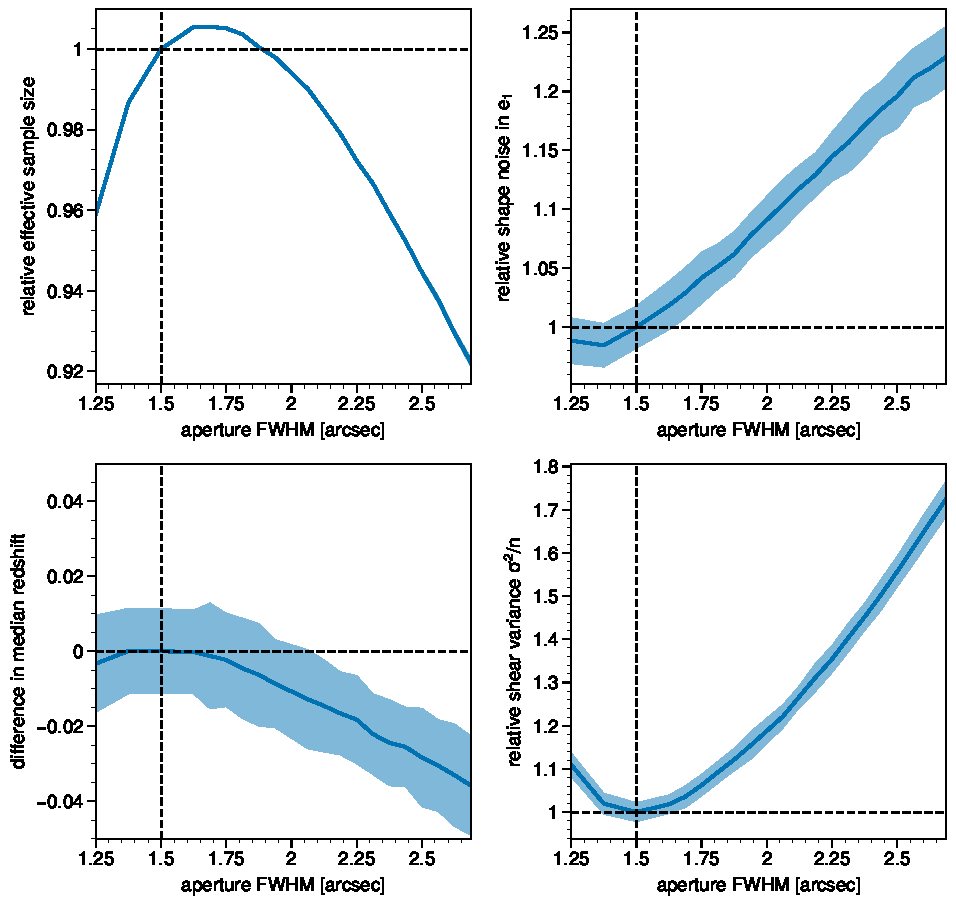
\includegraphics[width=\columnwidth]{figures/optap.pdf}
  \caption{
    Optimal Aperture for Pre-PSF Gaussian Moments. We show the relative effective sample
    size (top-left), the relative effective shape noise (top-right), the change in the median
    redshift (bottom-left), and relative total shear variance (bottom-right). All quantities are
    relative to the optimal aperture of $\approx$1.5'' FWHM. The bands are $3\sigma$ uncretainties
    obtained through bootstrap resampling. The optimum is determined by a trade-off
    between the effective shape noise and the effective number density, and it does not appear to
    result in a significant loss of redshift depth.
    \label{fig:opap}
  }
\end{figure}

We start by determining the optimal measurement aperture. For this task, we simulate
isolated objects. We then compute our moments statistics for a range of apertures between 1.25''
to 2.75''. For each aperture, we employ a set of cuts on the objects that mimics a typical weak lensing
sample selection using \mdet. These cuts are
\begin{eqnarray}
& {\rm flags} = 0 & \nonumber \\
& {\rm flux\ S/N} > 10 & \nonumber \\
& {\rm T/T_{psf}} > 0.5 & \nonumber
\end{eqnarray}
We then compute an inverse variance weight per object as
\begin{equation}
w = \frac{1}{\Delta e^2 + \sigma_e^2}
\end{equation}
where $\sigma_e$ is the raw shape noise of the sample with cuts applied and $\Delta e$ is
the pixel noise induced error on the shape measurement. Finally, we compute a set of
weak lensing sample statistics including the total sample size with cuts,
the effective number density
\begin{equation}
n_{\rm eff} = \frac{\left(\sum w\right)^2}{\sum w^2}\ ,
\end{equation}
the effective shape noise
\begin{equation}
\sigma_{e,{\rm eff}}^2 = \frac{\sum (we)^2}{\left(\sum w\right)^2}\ ,
\end{equation}
and overall total shear variance $\sigma_{e,{\rm eff}}^2/n_{\rm eff}$. See \mrb{cite heymans}
for the details of these shape measurement statistics.

We show the results of these computations in Figure~\ref{fig:opap}. We find that the
minimal total shear variance is achieved with an aperture of $\approx$1.5'' FWHM (bottom-right panel).
In the top-left panel, we show the effective sample size scaled relative to the sample
size at the optimal aperture. We show the effective shape noise and difference in the
median redshift of the selected sample also relative to optimal aperture in the top-right and
bottom-left panels respectively. As expected, the optimal sample is a trade off between
larger apertures which increase the sample size and smaller apertures which decrease
the shape noise. We find that the median redshift of the sample has a fairly broad peak
around the optimal aperture, indicating that the optimal aperture in terms of the total
shear variance is not sacrificing redshift depth.


\begin{figure}
  \centering
  \vspace{1em}
  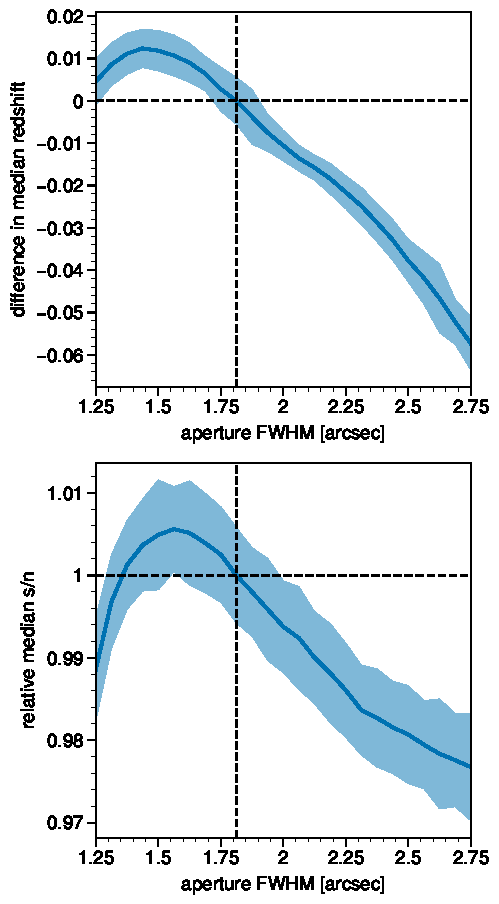
\includegraphics[width=\columnwidth]{figures/optap_depth.pdf}
  \caption{
    Optimal Aperture for Depth fot Pre-PSF Gaussian Moments.
    \label{fig:opap_depth}
  }
\end{figure}


\subsection{Error Properties for Isolated Objects}

We next examine the error properties of these estimators for isolated objects. We have not
studied blending in detail since it has obvious effects that are well beyond the capacity
of these estimators to recover and are common to all fixed aperture object measures. For this task,
we use the same isolated object simulations and an aperture size of 1.5'' FWHM. We obtain the
true flux in our selected aperture by running both a noiseless and noisy simulation for each
object. The results of our simulations, binned by true signal-to-noise are shown in
Figure~\ref{fig:noround_nodetect}. In the top panel, we show the fraction of flux recovered
as a function of signal-to-noise. This fraction depends on both the size of our aperture
and the object's profile. In particular, the profiles of objects in an LSST-like survey
are a function of signal-to-noise, generating the observed recovered flux trend. In the middle
panel, we show the fractional bias in the aperture flux measurement. We find that our code
recovers the true aperture flux to better than 1\%. Finally in the bottom panel, we show
the fractional difference between our reported flux errors and the empirical flux error
measured from the difference between our flux measurements and the true aperture flux. We
find that our reported flux errors are accurate to better than a few percent.

\begin{figure}
  \centering
  \vspace{1em}
  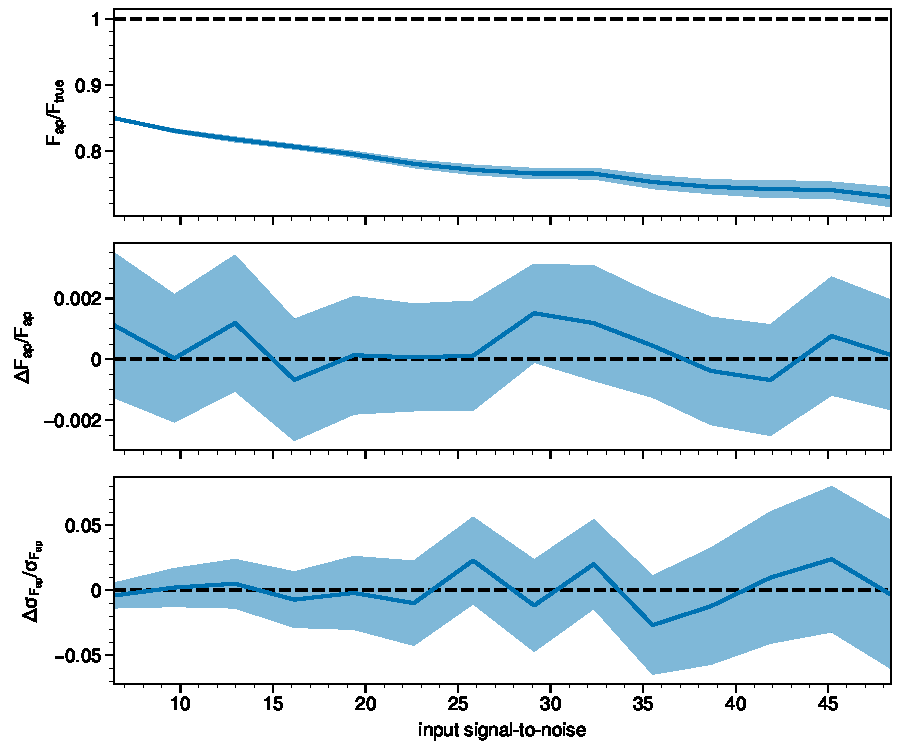
\includegraphics[width=\columnwidth]{figures/test-noround-nodetect.pdf}
  \caption{
    Statistics for Isolated Object Measurements. In the top panel, we show the
    fraction fo flux recovered for a typical object as a function of signal-to-noise.
    As expected, because our fixed Gaussian apertures are not matched to the objects,
    we typically underestimate the total flux. The degree of underestimation depends on
    the true profile of the object which changes systematically as a function of
    signal-to-noise in our simulations. In the middle panel, we show the fractional bias in
    our aperture flux measurement. Finally, in the bottom panel,
    we show the fractional deviation of our flux error predictions from the true
    empirical scatter in the flux. The bands in each panel show the $3\sigma$ uncertainties
    in our measurements obtained from bootstrap resampling. For isolated objects
    with white pixel noise, our reported measurements and errors are correct to
    better than a few percent.
    \label{fig:noround_nodetect}
  }
\end{figure}


\subsection{Shear Recovery Under Blending with \mdet}

Finally we evaluate how well our moments estimates work with \mdet. For this test,
we simulate pairs of exponential objects with a half-light radius of 0.5'' and a
signal-to-noise of $\approx20$ with the same PSF as above. We then run \mdet using our \pgauss
moments as the shape measurement. We measure the multiplicative bias, shear response, and
number of objects detected as a function of the separation of the pair. The results
of this test are show in Figure~\ref{fig:shearpair}. We find that the multiplicative
bias is consistent with second order shear effects, but that as detection
becomes maximally ambiguous (i.e., we detect 1.5 objects on average), there are large
changes in the shear response. We do find evidence for a slight increase on the
multiplicative bias near the maximally ambiguous case. This effect is not specific to \pgauss
and was documented in \mrb{cite} for the case of a post-PSF Gaussian moment.

\begin{figure}
  \centering
  \vspace{1em}
  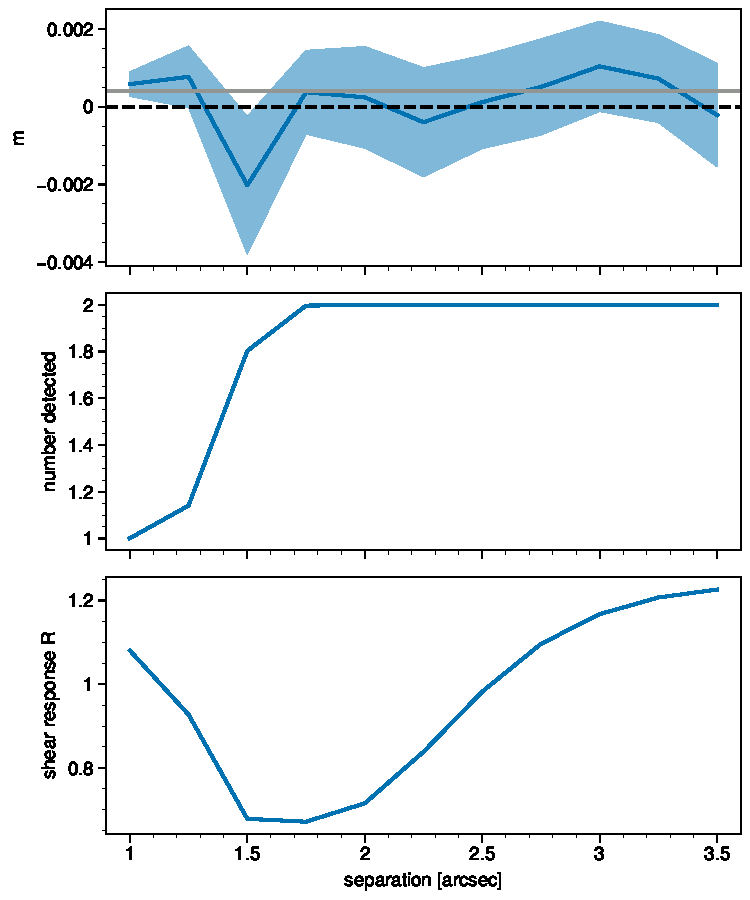
\includegraphics[width=\columnwidth]{figures/pair-plot.pdf}
  \caption{
    Tests of shear recovery for pairs of galaxies. On the top panel, we show
    the multiplicative bias for pairs of exponential objects as a function of
    the separation of the pair of the pair. These objects have a half-light radius
    of 0.5'' and a signal-to-noise of $\approx 20$. We also show the expected multiplicative
    bias from second-order shear effects as the grey solid line. In the middle panel, we show
    the average number of objects detected. In the bottom panel, we show the
    \mdet response of the objects to shear. The bands about each line, some not
    visible, show the 3$\sigma$ errors from bootstrap resampling. As blending
    causes the maximum ambiguity in detection (i.e., the mean number of detections
    is $\approx 1.5$), we see systematic changes in the response and a slight
    increase in the overall multiplicative bias from \mdet. This effect for our
    moments is no worse than the post-PSF weighted moments used in % \citep{sheldon2020}.
    \label{fig:shearpair}
  }
\end{figure}

\section{Summary}\label{sec:conc}


\section*{Acknowledgments}

ESS is supported by DOE grant DE-AC02-98CH10886, and MRB is supported by DOE
grant DE-AC02-06CH11357.  We gratefully acknowledge the computing resources
provided on Bebop, a high-performance computing cluster operated by the
Laboratory Computing Resource Center at Argonne National Laboratory, and the
RHIC Atlas Computing Facility, operated by Brookhaven National Laboratory.

\bibliographystyle{aasjournal}
\bibliography{references}

% \appendix

\end{document}
